\graphicspath{{chapters/5_experimentos/figures/}}

\chapter{Experimentación}\label{chap:experiments}

Para analizar el rendimiento de la implementación, se realizaron experimentos en distintas tarjetas gráficas, las cuales se ven en el cuadro \ref{tab:hardware-used}.
Estas, $H1$, $H2$ y $H3$, corresponden a hardware con capacidades gráficas progresivamente superiores.
Las escenas utilizadas se muestran en las figuras \ref{fig:cornell-box-full} y \ref{fig:sponza}, que llamaremos $S1$ y $S2$ respectivamente.
Se puede observar en cada una de ellas la luz indirecta difusa, luz indirecta especular y sombras suaves.

\begin{table}[ht]
	\centering
	\begin{tabular}{|c|c|c|c|c|}
		\hline
		\textbf{Nombre} & \textbf{GPU} & \textbf{Núcleos} & \textbf{Clock (GHz)} & \textbf{VRAM (GB)} \\
		\hline
		$H1$ & Intel Mesa ADL GT2 & 96 & 1.45 & * \\
		\hline
		$H2$ & Nvidia GTX 1660 Ti mobile & 1536 & 1.45 & 6 \\
		\hline
		$H3$ & Nvidia Geforce RTX 4070 & 5888 & 1.92 & 12 \\
		\hline
	\end{tabular}
	\caption{Hardware utilizado. * al ser una tarjeta integrada, no tiene memoria gráfica dedicada.}
	\label{tab:hardware-used}
\end{table}

\begin{figure}[H]
	\centering
	  \begin{subfigure}{0.49\textwidth}
	      \centering
	  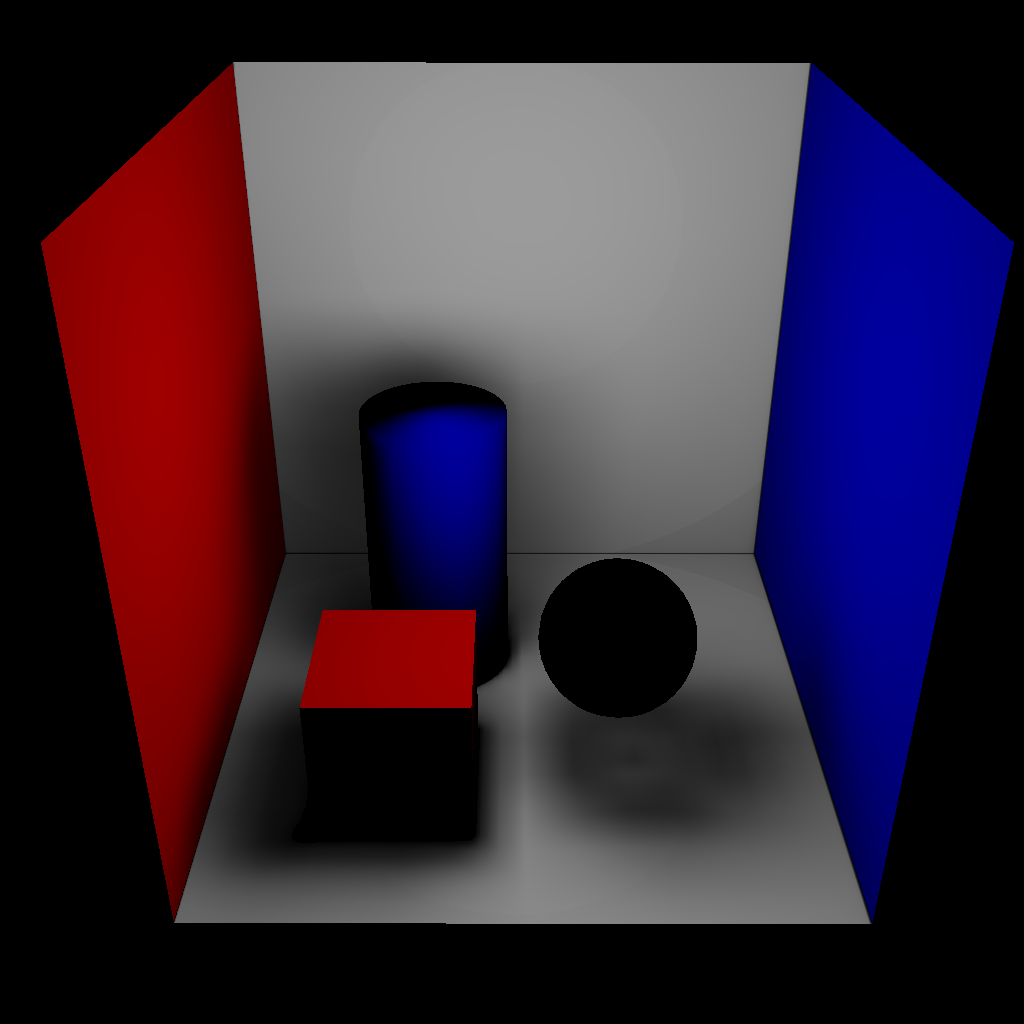
\includegraphics[width=\textwidth]{cornell-box-direct.png}
	      \caption{Solo luz directa.}
	  \end{subfigure}
	  \begin{subfigure}{0.49\textwidth}
	      \centering
	  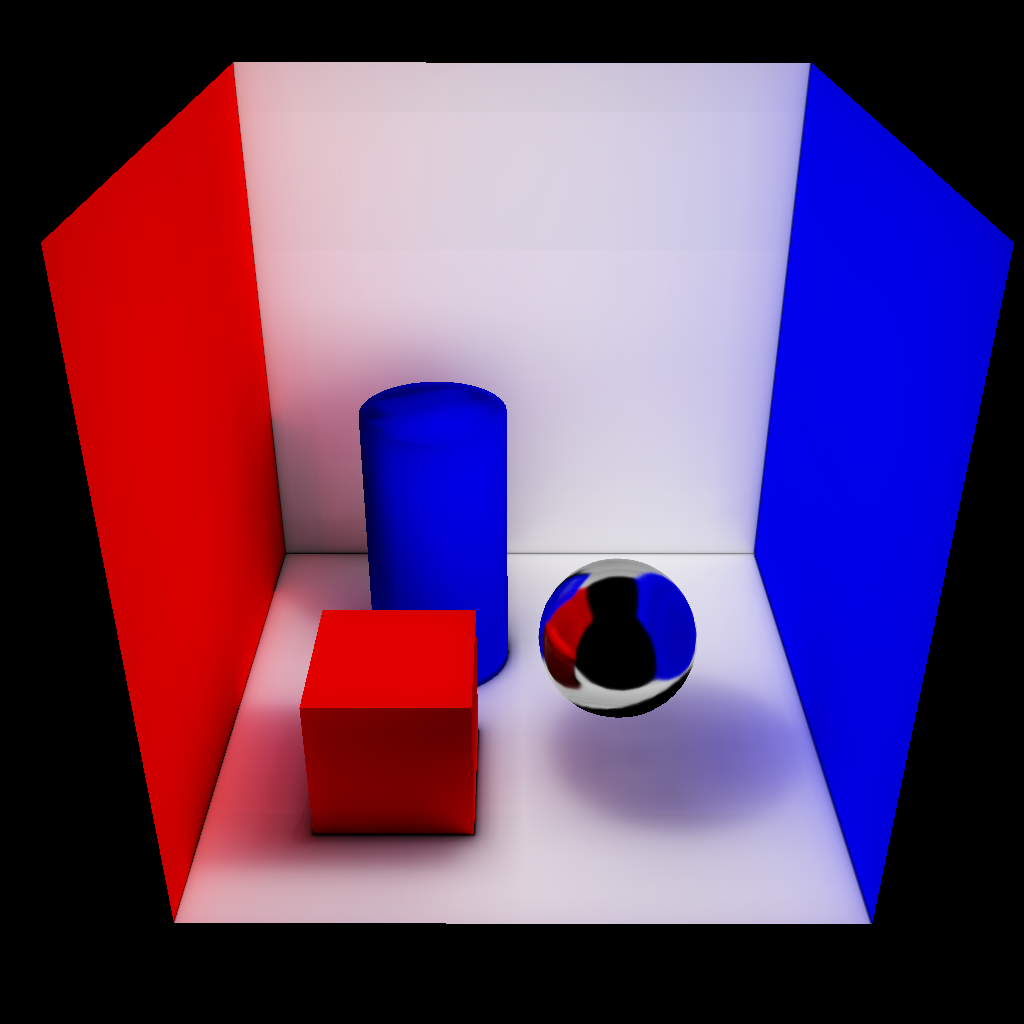
\includegraphics[width=\textwidth]{cornell-box-full.png}
	      \caption{Luz directa e indirecta.}
	  \end{subfigure}
	\caption{Escena de prueba con geometría simple.}
	\label{fig:cornell-box-full}
\end{figure}

\begin{figure}[H]
	\begin{subfigure}{0.49\textwidth}
	  \centering
	  \includegraphics[width=\textwidth]{sponza-direct.png}
	  \caption{Solo luz directa.}
	\end{subfigure}
	\begin{subfigure}{0.49\textwidth}
	  \centering
	  \includegraphics[width=\textwidth]{sponza-all.png}
	  \caption{Luz directa e indirecta.}
	\end{subfigure}
	\caption{Sponza.}
	\label{fig:sponza}
\end{figure}

Los experimentos varían la cantidad de vóxeles por dimensión, y registran los cuadros por segundo alcanzados (FPS, por sus siglas en inglés) y el tiempo de construcción del \textit{octree} en segundos.
Para conseguir los FPS se ejecutó el programa durante un minuto, tomando una muestra cada segundo, luego se promediaron.
Para el tiempo de construcción del \textit{octree}, se construyó 50 veces y se calculó el tiempo promedio.
Cada ejecución se realizó independientemente, para evitar posibles mejoras debido al uso del cache.

En el cuadro \ref{tab:experiment-results} se muestran los resultados de estos experimentos en los 3 hardwares utilizados ($H1$, $H2$ y $H3$) descritos en el cuadro \ref{tab:hardware-used}.
Se muestran los resultados para cada una de las escenas $S1$ y $S2$, en cada uno de los hardwares, y para cada nivel de resolución (vóxeles por dimensión).

\begin{table}[ht]
\centering
\begin{tabular}{|c|c|c|c|c|}
	\hline
	\textbf{Escena} & \textbf{Hardware} & \textbf{Vóxeles} & \textbf{FPS} & \textbf{Construcción del \textit{octree} (s)} \\
	\hline
	$S1$ & $H1$ & $256$ & $18.22$ & $1.76$ \\
	\cline{3-5}
	 & & $512$ & $14.77$ & $1.82$ \\
	\cline{3-5}
	 & & $1024$ & $12.13$ & $2.01$ \\
	\cline{2-5}
	 & $H2$ & $256$ & $136.57$ & $1.78$ \\
	\cline{3-5}
	 & & $512$ & $108.67$ & $1.80$ \\
	\cline{3-5}
	 & & $1024$ & $60.24$ & $1.89$ \\
	\cline{2-5}
	 & $H3$ & $256$ & $141.57$ & $1.88$ \\
	\cline{3-5}
	 & & $512$ & $141.47$ & $1.90$ \\
	\cline{3-5}
	 & & $1024$ & $140.88$ & $1.89$ \\
	\hline
	$S2$ & $H1$ & $256$ & $7.30$ & $1.84$ \\
	\cline{3-5}
	 & & $512$ & $4.29$ & $1.86$ \\
	\cline{3-5}
	 & & $1024$ & $2.84$ & $2.07$ \\
	\cline{2-5}
	 & $H2$ & $256$ & $59.68$ & $1.82$ \\
	\cline{3-5}
	 & & $512$ & $37.42$ & $1.94$ \\
	\cline{3-5}
	 & & $1024$ & $9.83$ & $1.83$ \\
	\cline{2-5}
	 & $H3$ & $256$ & $141.27$ & $1.70$ \\
	\cline{3-5}
	 & & $512$ & $141.51$ & $1.91$ \\
	\cline{3-5}
	 & & $1024$ & $141.21$ & $1.99$ \\
	\hline
\end{tabular}
\caption{FPS y tiempo de construcción del octree para cada escena.}
\label{tab:experiment-results}
\end{table}

\section{Análisis de resultados}

Una primera observación es que los cuadros por segundo se encuentran cerca del tiempo real.
Se nota que en $H1$ los FPSs nunca superan los 20, mientras que en $H3$ nunca bajan de 140.
$H2$ representa un término medio, logrando más de 60 FPS en la escena simple ($S1$) y mostrando una gran variedad de valores en la escena compleja ($S2$) para cada resolución utilizada ($256$, $512$, $1024$).

Se observa que, como es de esperarse, a mayor resolución (vóxeles por dimensión), los cuadros por segundo disminuyen.
Esto se debe a que una resolución más alta mejora la aproximación y genera imágenes de mayor calidad, pero a costa de mayor carga computacional.

Un aspecto que destaca especialmente es el tiempo de construcción del octree, que permanece alrededor de los 2 segundos, cuando idealmente debería estar en el rango de los milisegundos.
Dado que este tiempo es prácticamente igual tanto en $H1$ como en $H3$, parece evidente que el cuello de botella no es la GPU en si, si no la comunicación entre GPU y CPU.
